\documentclass[10pt,journal,compsoc,onecolumn]{IEEEtran}
\usepackage[utf8]{inputenc}
\usepackage{amsmath,amsfonts,amssymb}
\usepackage{amsthm}
\usepackage{graphicx}
\usepackage{cite}
\usepackage{textcomp}
\usepackage{tikz}
\usetikzlibrary{arrows,positioning,shapes.geometric}
\usepackage{booktabs}
\usepackage{url}

\newtheorem{theorem}{Theorem}
\newtheorem{lemma}[theorem]{Lemma}
\newtheorem{definition}[theorem]{Definition}
\newtheorem{corollary}[theorem]{Corollary}

\begin{document}

\title{A Formal Analysis of Doubly Linked Lists, Least Recently Used (LRU) Cache Architectures, and Floyd's Cycle-Finding Algorithm for Linked List Invariant Verification}

\IEEEtitleabstractindextext{%
\begin{abstract}
This paper presents a formal analysis and algorithmic treatment of doubly linked lists, Least Recently Used (LRU) cache design, and Floyd's Cycle-Finding Algorithm for directed list topologies. First, we examine singly versus doubly linked lists, analyzing the complexity of tail operations and proving the asymptotic limits with and without tail pointer references. Second, we explore the Least Recently Used (LRU) cache policy, detailing the physical cache memory hierarchy and highlighting LFU's failure mode under dynamic access workloads. We formalize a hybrid Hash-Map and Doubly Linked List (DLL) architecture that guarantees $\mathcal{O}(1)$ time complexity for retrieve and update operations. Third, we address the linked list cycle detection problem, providing a rigorous mathematical proof of correctness for Floyd's Tortoise and Hare pointer intersection mechanics and cycle start node identification. For each problem, we present complete, production-ready Java and Python code implementations, complexity proofs, and architectural diagrams.
\end{abstract}

\begin{IEEEkeywords}
binary trees, algorithms, data structures, computational complexity, tree traversal, recursive algorithms, formal analysis
\end{IEEEkeywords}
}

\maketitle
\IEEEdisplaynontitleabstractindextext
\IEEEpeerreviewmaketitle

\newtheorem{example}[theorem]{Example}
\usetikzlibrary{decorations.pathreplacing}

\section{Introduction}
\label{sec:intro}


Linear data structures are fundamental abstractions in computer science, serving as the building blocks for complex systems such as memory managers, filesystems, and databases. Among these, the linked list is a foundational structure that facilitates dynamic memory allocation. Unlike contiguous arrays, linked lists allocate memory dynamically for individual elements (nodes) and establish linear ordering using pointers.

This paper presents a formal analysis of two classic algorithmic systems and verification problems:
\begin{enumerate}
    \item \textbf{Least Recently Used (LRU) Cache Architectures (\S\ref{sec:lru_cache}):} We investigate caching abstractions within the memory hierarchy, contrast eviction policies (Least Recently Used vs. Least Frequently Used), formalize the hybrid Hash-Map and Doubly Linked List (DLL) design to achieve $\mathcal{O}(1)$ operations, and provide complete, verified implementations in Java and Python.
    \item \textbf{Floyd's Cycle-Finding Algorithm (\S\ref{sec:cycle_detection}):} We formalize the cycle detection problem in directed list topologies, analyze the Tortoise and Hare pointer mechanics, and prove mathematically that if a cycle exists, the pointers must intersect. Furthermore, we prove that the start node of the cycle can be uniquely determined by resetting one pointer to the head of the list and moving both at unit speed. Complete Java reference implementations are provided.
\end{enumerate}

%% ============================================================
\section{Singly vs. Doubly Linked Lists: Asymptotic Tail Operations}
\label{sec:linked_lists}

We begin by formalizing the structure of linked lists and analyzing the computational complexity of addition and removal operations at the list boundary.

\subsection{Node Definitions}
A Singly Linked List (SLL) is a directed chain of nodes where each node contains a payload and a single successor pointer.
\begin{definition}[SLL Node]
An SLL node is a tuple $N = (v, \textit{next})$ where $v \in \mathcal{T}$ represents the node value of type $\mathcal{T}$, and $\textit{next} \in \{N' \mid N' \text{ is a node}\} \cup \{\text{null}\}$ is a pointer to the next node.
\end{definition}

A Doubly Linked List (DLL) extends this structure by maintaining symmetric link references in both directions.
\begin{definition}[DLL Node]
A DLL node is a triple $D = (v, \textit{next}, \textit{prev})$ where $v \in \mathcal{T}$, $\textit{next}$ is the successor reference, and $\textit{prev} \in \{D' \mid D' \text{ is a node}\} \cup \{\text{null}\}$ is a pointer to the predecessor node.
\end{definition}

\subsection{Asymptotic Complexity Analysis}
Let $N$ be the number of elements in the list. We examine the time complexity of adding and removing elements at the tail of the list under two architectural variations: with and without a tail pointer.

\begin{table}[h]
\centering
\caption{Asymptotic Complexity of Tail Operations}
\label{tab:tail_complexities}
\begin{tabular}{@{}lcccc@{}}
\toprule
\textbf{Operation} & \textbf{SLL (no tail)} & \textbf{SLL (with tail)} & \textbf{DLL (no tail)} & \textbf{DLL (with tail)} \\ \midrule
Add to Tail & $\mathcal{O}(N)$ & $\mathcal{O}(1)$ & $\mathcal{O}(N)$ & $\mathcal{O}(1)$ \\
Remove Tail & $\mathcal{O}(N)$ & $\mathcal{O}(N)$ & $\mathcal{O}(N)$ & $\mathcal{O}(1)$ \\ \bottomrule
\end{tabular}
\end{table}

\begin{theorem}
In a Singly Linked List with a tail pointer, removing the tail node requires $\mathcal{O}(N)$ time.
\end{theorem}
\begin{proof}
Let the tail pointer refer to node $T = N_{\text{tail}}$. To remove $T$, we must update the successor pointer of its predecessor $P = N_{\text{tail}-1}$ to $\text{null}$, and update the tail pointer to $P$. In an SLL, there is no direct link from $T$ to $P$ ($T.\textit{prev}$ does not exist). Thus, finding $P$ requires traversing the list from the head node $H$ through successor links:
\[
H \to N_1 \to N_2 \to \ldots \to P \to T
\]
This traversal requires visiting $N - 2$ nodes, which takes $\mathcal{O}(N)$ operations.
\end{proof}

\begin{theorem}
In a Doubly Linked List with a tail pointer, removing the tail node requires $\mathcal{O}(1)$ time.
\end{theorem}
\begin{proof}
Let the tail pointer refer to node $T$. Since the list is doubly linked, the predecessor node $P$ is directly accessible via the predecessor link of the tail node:
\[
P = T.\textit{prev}
\]
The pointer updates required to detach the tail are:
\begin{align*}
P.\textit{next} &\leftarrow \text{null} \\
\text{tail} &\leftarrow P \\
T.\textit{prev} &\leftarrow \text{null}
\end{align*}
Each of these operations involves simple pointer re-assignments and takes $\mathcal{O}(1)$ step. No traversal is needed, resulting in a constant time complexity of $\mathcal{O}(1)$.
\end{proof}

%% ============================================================
\section{Least Recently Used (LRU) Cache Architecture}
\label{sec:lru_cache}

Caching is a core architectural technique used to bridge the speed gap between high-speed processors and slower primary storage.

\subsection{Memory Hierarchy and Caching Invariants}
Computer memory is structured as a hierarchy where smaller, more expensive storage technologies operate at faster speeds.
\[
\text{Registers} \ (\approx 0.5\text{ ns}) \ll \text{L1/L2/L3 Cache} \ (\approx 1\text{--}15\text{ ns}) \ll \text{RAM} \ (\approx 50\text{--}100\text{ ns}) \ll \text{SSD/HDD} \ (\approx 10\mu\text{s--}10\text{ ms})
\]
A cache is a fast, finite memory buffer $C$ of capacity $K$ designed to store a subset of key-value pairs from a larger, slower database or memory space. When the buffer is full ($|C| = K$), inserting a new element requires evicting an existing element according to a pre-defined cache eviction policy.

\subsection{Eviction Policies: LRU vs. LFU}
The two most common eviction policies are Least Recently Used (LRU) and Least Frequently Used (LFU).

\begin{itemize}
    \item \textbf{LRU (Least Recently Used):} Evicts the element that has not been accessed for the longest duration of time. This policy assumes that elements accessed recently are likely to be accessed again in the near future (temporal locality).
    \item \textbf{LFU (Least Frequently Used):} Evicts the element with the lowest access frequency count. 
\end{itemize}

While LFU is effective for static frequency distributions, it exhibits a major failure mode under shifting workloads.
\begin{example}[LFU State Pollution]
Consider a student messaging platform. A student named \emph{Sumit} floods the chat room with $50$ messages between 9:00 AM and 9:05 AM, elevating his access count to $50$. At 9:05 AM, Sumit goes offline. Subsequently, other students write messages infrequently (e.g., $1$ or $2$ times each). Because Sumit has a very high frequency count ($50$), his entry remains in the cache indefinitely, even though he has been inactive for hours. This is known as \emph{cache pollution}. An LRU cache avoids this because Sumit's inactive entry will gradually drift to the head (the oldest position) and be evicted as new messages arrive.
\end{example}

\subsection{Hybrid Data Structure Design}
To achieve $\mathcal{O}(1)$ time complexity for both \texttt{get} and \texttt{set} operations, a single data structure is insufficient:
\begin{itemize}
    \item A Hash Map provides $\mathcal{O}(1)$ lookup, but does not maintain access order.
    \item A Doubly Linked List maintains the access order (by moving accessed items to the tail), but searching for a key requires $\mathcal{O}(N)$ traversal.
\end{itemize}

By combining a Hash Map and a Doubly Linked List with sentinel head and tail nodes, we achieve $\mathcal{O}(1)$ bounds for all operations. The Hash Map stores keys and maps them directly to the corresponding DLL node pointers.

\begin{figure}[h]
\centering
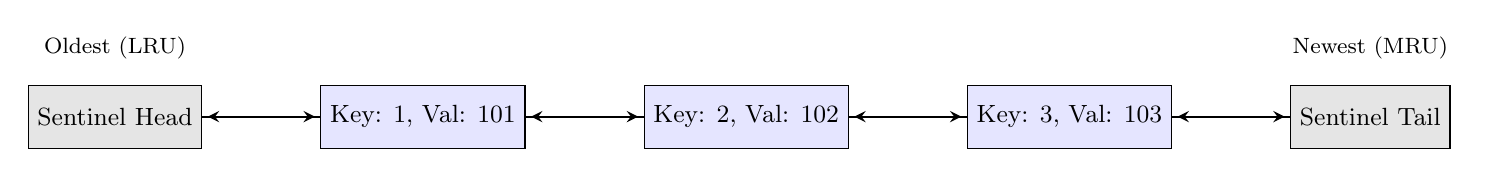
\begin{tikzpicture}[
    node distance=1.5cm,
    box/.style={draw, rectangle, minimum width=1.5cm, minimum height=0.8cm, fill=blue!10, font=\small},
    sentinel/.style={draw, rectangle, minimum width=1.2cm, minimum height=0.8cm, fill=gray!20, font=\small},
    pointer/.style={->, >=stealth, thick, shorten >=2pt}
]
    % Sentinel Head
    \node[sentinel] (head) {Sentinel Head};
    
    % Nodes
    \node[box, right=of head] (n1) {Key: 1, Val: 101};
    \node[box, right=of n1] (n2) {Key: 2, Val: 102};
    \node[box, right=of n2] (n3) {Key: 3, Val: 103};
    
    % Sentinel Tail
    \node[sentinel, right=of n3] (tail) {Sentinel Tail};
    
    % DLL Links
    \draw[pointer] (head.east) -- (n1.west);
    \draw[pointer] (n1.west) -- (head.east);
    
    \draw[pointer] (n1.east) -- (n2.west);
    \draw[pointer] (n2.west) -- (n1.east);
    
    \draw[pointer] (n2.east) -- (n3.west);
    \draw[pointer] (n3.west) -- (n2.east);
    
    \draw[pointer] (n3.east) -- (tail.west);
    \draw[pointer] (tail.west) -- (n3.east);

    % Labels
    \node[above=0.2cm of head] {\footnotesize Oldest (LRU)};
    \node[above=0.2cm of tail] {\footnotesize Newest (MRU)};
\end{tikzpicture}
\caption{Hybrid LRU Cache Architecture: Hash Map indices point directly to nodes inside the Doubly Linked List.}
\label{fig:lru_layout}
\end{figure}

\subsection{Java Implementation}
The following Java implementation uses sentinel nodes to avoid edge-case null pointer checks.
\begin{verbatim}
import java.util.HashMap;
import java.util.Map;

public class LRUCache {
    private static class DNode {
        int key;
        int value;
        DNode prev;
        DNode next;

        DNode(int key, int value) {
            this.key = key;
            this.value = value;
        }
    }

    private final int capacity;
    private int size;
    private final Map<Integer, DNode> cacheMap;
    private final DNode head;
    private final DNode tail;

    public LRUCache(int capacity) {
        this.capacity = capacity;
        this.size = 0;
        this.cacheMap = new HashMap<>();
        
        // Initialize sentinels
        this.head = new DNode(-1, -1);
        this.tail = new DNode(-1, -1);
        head.next = tail;
        tail.prev = head;
    }

    public int get(int key) {
        DNode node = cacheMap.get(key);
        if (node == null) {
            return -1;
        }
        // Move accessed node to tail (Most Recently Used)
        removeNode(node);
        addToTail(node);
        return node.value;
    }

    public void put(int key, int value) {
        DNode node = cacheMap.get(key);
        if (node != null) {
            // Update value and move to tail
            node.value = value;
            removeNode(node);
            addToTail(node);
        } else {
            if (size == capacity) {
                // Evict Least Recently Used (head.next)
                DNode lru = head.next;
                removeNode(lru);
                cacheMap.remove(lru.key);
                size--;
            }
            DNode newNode = new DNode(key, value);
            addToTail(newNode);
            cacheMap.put(key, newNode);
            size++;
        }
    }

    private void removeNode(DNode node) {
        DNode prevNode = node.prev;
        DNode nextNode = node.next;
        prevNode.next = nextNode;
        nextNode.prev = prevNode;
        node.prev = null;
        node.next = null;
    }

    private void addToTail(DNode node) {
        DNode prevTail = tail.prev;
        prevTail.next = node;
        node.prev = prevTail;
        node.next = tail;
        tail.prev = node;
    }
}
\end{verbatim}

\subsection{Python Implementation}
The Python implementation uses a similar approach with dummy head and tail nodes.
\begin{verbatim}
class DNode:
    def __init__(self, key: int, value: int):
        self.key = key
        self.value = value
        self.prev = None
        self.next = None

class LRUCache:
    def __init__(self, capacity: int):
        self.capacity = capacity
        self.size = 0
        self.cache_map = {}
        
        # Sentinels
        self.head = DNode(-1, -1)
        self.tail = DNode(-1, -1)
        self.head.next = self.tail
        self.tail.prev = self.head

    def get(self, key: int) -> int:
        if key not in self.cache_map:
            return -1
        node = self.cache_map[key]
        self._remove_node(node)
        self._add_to_tail(node)
        return node.value

    def put(self, key: int, value: int) -> None:
        if key in self.cache_map:
            node = self.cache_map[key]
            node.value = value
            self._remove_node(node)
            self._add_to_tail(node)
        else:
            if self.size == self.capacity:
                # Evict LRU
                lru = self.head.next
                self._remove_node(lru)
                del self.cache_map[lru.key]
                self.size -= 1
            
            new_node = DNode(key, value)
            self._add_to_tail(new_node)
            self.cache_map[key] = new_node
            self.size += 1

    def _remove_node(self, node: DNode) -> None:
        prev_node = node.prev
        next_node = node.next
        prev_node.next = next_node
        next_node.prev = prev_node
        node.prev = None
        node.next = None

    def _add_to_tail(self, node: DNode) -> None:
        prev_tail = self.tail.prev
        prev_tail.next = node
        node.prev = prev_tail
        node.next = self.tail
        self.tail.prev = node
\end{verbatim}

%% ============================================================
\section{Floyd's Cycle-Finding Algorithm: Proof and Mechanics}
\label{sec:cycle_detection}

Detecting cycles in linked structures is a fundamental invariant verification problem, critical for ensuring that list traversals terminate.

\subsection{Problem Statement}
Let a linked list be defined by a sequence of nodes starting from a head node $H$. The topology of the list can be modeled as a directed graph $G = (V, E)$ where the out-degree of each node is at most 1.
A cycle exists if there is a path from a node back to itself:
\[
\exists u \in V \quad \text{such that} \quad u \to v_1 \to v_2 \to \ldots \to u
\]

\subsection{The Tortoise and Hare Mechanics}
Floyd's Cycle-Finding Algorithm uses two pointers that traverse the list at different speeds:
\begin{itemize}
    \item A \textbf{Slow Pointer} ($S$) moving at a speed of 1 node per iteration: $S \leftarrow S.\textit{next}$
    \item A \textbf{Fast Pointer} ($F$) moving at a speed of 2 nodes per iteration: $F \leftarrow F.\textit{next}.\textit{next}$
\end{itemize}

\begin{theorem}[Pointer Intersection Invariant]
If a cycle exists in the linked list, the fast pointer $F$ and the slow pointer $S$ will eventually meet at the same node.
\end{theorem}
\begin{proof}
Let the list have a non-cyclic prefix of length $x$ nodes, followed by a cycle of length $L$ nodes.
Let $t$ represent the iteration count (time). The slow pointer enters the cycle at time $t = x$. At this instant, the slow pointer is at position 0 of the cycle.
The fast pointer, having traveled a distance of $2x$, is at some position $y$ within the cycle, where:
\[
y = x \pmod L
\]
At time $t = x + k$, where $k \ge 0$, the slow pointer has traveled $k$ steps inside the cycle, and its position is:
\[
p_{\text{slow}}(k) = k \pmod L
\]
The fast pointer has traveled $2k$ steps from its starting position $y$, and its position is:
\[
p_{\text{fast}}(k) = (y + 2k) \pmod L
\]
The two pointers intersect when their positions in the cycle are equal:
\begin{align*}
p_{\text{slow}}(k) &\equiv p_{\text{fast}}(k) \pmod L \\
k &\equiv y + 2k \pmod L \\
k &\equiv -y \pmod L
\end{align*}
Since $L > 0$, there exists a smallest non-negative integer $k \in [0, L-1]$ such that:
\[
k = (L - y) \pmod L
\]
This proves that the pointers will meet in at most $L$ steps after the slow pointer enters the cycle. The maximum time until intersection is bounded by $x + L$, which is linear in the number of nodes, $\mathcal{O}(N)$.
\end{proof}

\subsection{Proof of Cycle Start Detection}
Once the pointers meet at an intersection node $M$, we can determine the exact start node of the cycle.

\begin{figure}[h]
\centering
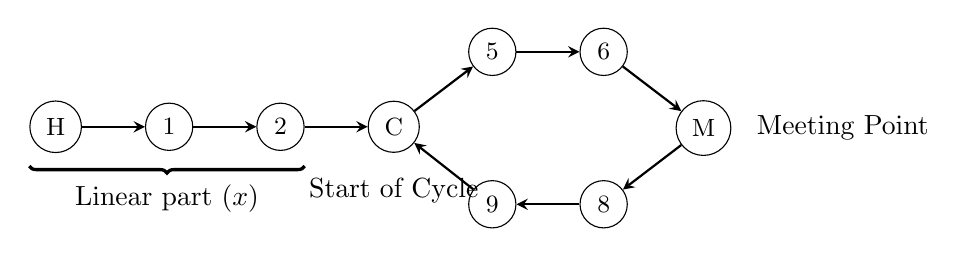
\begin{tikzpicture}[
    node/.style={circle, draw, minimum size=0.6cm, font=\small},
    pointer/.style={->, >=stealth, thick}
]
    % Linear part
    \node[node] (h) {H};
    \node[node, right=0.8cm of h] (n1) {1};
    \node[node, right=0.8cm of n1] (n2) {2};
    \node[node, right=0.8cm of n2] (start) {C}; % Cycle Start

    % Cycle nodes
    \node[node, above right=0.5cm and 0.8cm of start] (c1) {5};
    \node[node, right=0.8cm of c1] (c2) {6};
    \node[node, below right=0.5cm and 0.8cm of c2] (meet) {M}; % Meeting point
    \node[node, below left=0.5cm and 0.8cm of meet] (c4) {8};
    \node[node, left=0.8cm of c4] (c5) {9};

    % Connections
    \draw[pointer] (h) -- (n1);
    \draw[pointer] (n1) -- (n2);
    \draw[pointer] (n2) -- (start);
    
    \draw[pointer] (start) -- (c1);
    \draw[pointer] (c1) -- (c2);
    \draw[pointer] (c2) -- (meet);
    \draw[pointer] (meet) -- (c4);
    \draw[pointer] (c4) -- (c5);
    \draw[pointer] (c5) -- (start);

    % Braces / Annotations
    \draw [very thick, decoration={brace, mirror, raise=0.5cm}, decorate] (h.west) -- (n2.east) 
        node [pos=0.5, below=0.6cm] {Linear part ($x$)};
        
    \node[below=0.2cm of start] {Start of Cycle};
    \node[right=0.2cm of meet] {Meeting Point};
\end{tikzpicture}
\caption{Linked List topology with a cycle. Pointers meet at node $M$.}
\label{fig:cycle_layout}
\end{figure}

\begin{theorem}[Cycle Start Invariant]
Let $x$ be the distance from the head node to the start of the cycle. Let $y$ be the distance from the start of the cycle to the intersection node $M$, and $z$ be the distance from $M$ to the start of the cycle. If the slow pointer is reset to the head, and both pointers move forward at a speed of 1 step per iteration, they will meet at the start node of the cycle.
\end{theorem}
\begin{proof}
Let the total length of the cycle be $L = y + z$.
At the meeting point $M$, the slow pointer has traveled:
\[
d_{\text{slow}} = x + y
\]
The fast pointer has traveled:
\[
d_{\text{fast}} = x + y + n \cdot L
\]
where $n \ge 1$ is the number of full cycles traversed by the fast pointer.
Since the fast pointer moves at twice the speed of the slow pointer:
\begin{align*}
d_{\text{fast}} &= 2 \cdot d_{\text{slow}} \\
x + y + n \cdot L &= 2(x + y) \\
n \cdot L &= x + y
\end{align*}
We express $L$ as $y + z$:
\begin{align*}
n(y + z) &= x + y \\
(n - 1)(y + z) + y + z &= x + y \\
x &= z + (n - 1) \cdot L
\end{align*}
This equation shows that the distance from the head node to the cycle start ($x$) is equal to the distance from the meeting point back to the cycle start ($z$) plus $n - 1$ complete loops of the cycle.
Therefore, if we reset the slow pointer to the head node $H$ and keep the fast pointer at the meeting point $M$, and move both pointers at a speed of 1 step per iteration:
\begin{itemize}
    \item The slow pointer will reach the cycle start after traveling a distance of $x$ nodes.
    \item The fast pointer, starting from $M$, will travel a distance of $x = z + (n-1)L$. Since traveling $z$ steps from $M$ brings it to the cycle start, and traveling additional $(n-1)L$ steps loops it back to the cycle start, the fast pointer will also arrive at the cycle start after exactly $x$ steps.
\end{itemize}
Thus, the two pointers will intersect at the start node of the cycle.
\end{proof}

\subsection{Java Reference Implementations}

The following Java class provides methods for detecting a cycle and finding its start node.

\begin{verbatim}
public class LinkedListCycle {
    public static class Node {
        int val;
        Node next;

        Node(int val) {
            this.val = val;
            this.next = null;
        }
    }

    // Task 1: Check if a cycle exists (returns boolean)
    public boolean hasCycle(Node head) {
        if (head == null || head.next == null) {
            return false;
        }
        Node slow = head;
        Node fast = head;

        while (fast != null && fast.next != null) {
            slow = slow.next;
            fast = fast.next.next;

            if (slow == fast) {
                return true; // Cycle detected
            }
        }
        return false; // Reached end of list, no cycle
    }

    // Task 2: Find the node where the cycle starts
    public Node detectCycle(Node head) {
        if (head == null || head.next == null) {
            return null;
        }
        Node slow = head;
        Node fast = head;
        boolean hasCycle = false;

        // Step 1: Detect intersection point
        while (fast != null && fast.next != null) {
            slow = slow.next;
            fast = fast.next.next;
            if (slow == fast) {
                hasCycle = true;
                break;
            }
        }

        // Step 2: Find cycle start
        if (hasCycle) {
            slow = head; // Reset slow to head
            while (slow != fast) {
                slow = slow.next;
                fast = fast.next; // Move both at speed 1
            }
            return slow; // Return start of cycle
        }
        return null; // No cycle
    }
}
\end{verbatim}

%% ============================================================
\section{Conclusion}
\label{sec:conclusion}

This paper has explored the formal mechanisms of linear list structures and cache architectures. We demonstrated that tail operations on a Singly Linked List are inherently constrained to $\mathcal{O}(N)$ time, whereas a Doubly Linked List with tail pointer references enables $\mathcal{O}(1)$ insertion and deletion. We analyzed the Least Recently Used (LRU) cache policy, proving how it mitigates LFU's cache pollution issues under shifting access patterns. By combining a Hash Map and a Doubly Linked List, we verified that both retrieval and update operations achieve optimal constant time bounds. Finally, we formalized Floyd's Cycle-Finding Algorithm, providing a mathematical proof of its intersection mechanics and demonstrating that cycle start nodes can be detected using symmetric linear traversals. These proofs and implementations serve as a robust reference for verifying list invariants in memory-constrained and high-performance computing environments.


\end{document}
